\documentclass{report}

\usepackage[italian]{babel}
\usepackage[utf8]{inputenc}
\usepackage[hidelinks]{hyperref}
\usepackage{graphicx}
\usepackage[font=small,labelfont=bf]{caption}
\graphicspath{ {../assets/} }

\title{Report sul protocollo GREEN-WUP}
\author{Leonardo Emili}

\begin{document}
\maketitle
\tableofcontents

\chapter{GREEN-WUP}
\section{Il protocollo GREEN-WUP}

Il protocollo GREEN-WUP si inserisce nel contesto dei protocolli delle cosiddette \emph{green wireless sensor network} e pone tra i suoi principali
obbiettivi l'efficienza energetica dell'intera rete. Esso impiega le tecnologie di wake up radio, energy harvesting e semantic addressing. Il protocollo è
di tipo \emph{converge casting} e fonda il suo funzionamento sull'assegnazione di hop count a ciascun nodo per poter distribuire i pacchetti dati
all'interno della rete.\\

Il protocollo è articolato in due fasi principali: in primo luogo avviene la fase di \emph{interest dissemination} si definisce la
topologia della rete da rispettare per realizzare affinchè i nodi realizzino un corretto flusso di scambio dati, successivamente si assume che gli indirizzi di
wake up siano stati assegnati e si procede con lo scambio di dati che è governato da sequenze di wake up usate per risvegliare i nodi della rete. \\

Inizialmente il sink node avvia la fase di interest dissemination inviando
un primo \emph{command packet} che viene successivamente distribuito ai nodi sensori utilizzando l'algoritmo di \emph{flooding}.
L'obbiettivo di questo processo è di assegnare a ciascun nodo della rete un valore di hop count secondo un algoritmo iterativo: in particolare questo
avrà valore 0 nel solo caso del sink node, altrimenti $h$ se $h-1$ è il valore di hop count del nodo precedente. Al termine
di questa fase ciascun nodo sarà fornito un indirizzo di wake up $w=w_{h}w_{e}$ della lunghezza di 8 bit , dove il prefisso $w_{h}$ è definito dalla
codifica in 4 bit di $h$ e $w_{e}$ rappresenta la classe energetica del nodo, codificata nei restanti 4 bit. In particolare, l'energia di un nodo viene
considerata relativamente all'energia rimamente nelle batterie e a quella derivata da sorgenti esterne. In definitiva, la codifica del suffisso $w_{e}$
viene calcolata a partire dalla discretizzazione in $k$ classi della disponibilità energetica di un nodo, dove $k$ rappresenta il numero delle classi
disponibili.\\

%image source: https://www.researchgate.net/figure/Topology-of-wireless-sensor-network-and-hop-count-of-sensors_fig7_285956270
\begin{figure}
    \begin{center}
        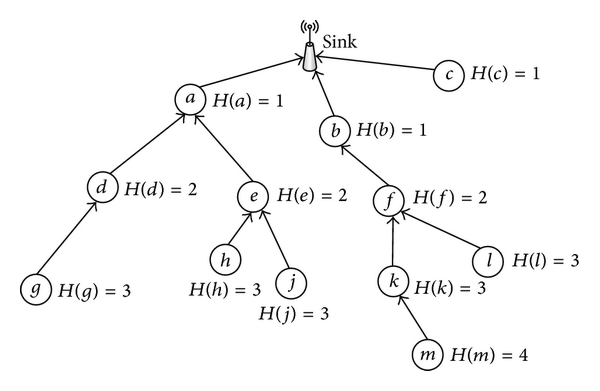
\includegraphics[scale=1.7]{hop-count-algorithm.png}
        \caption{Topologia della rete a seguito dell'assegnazione degli hop count}
    \end{center}
\end{figure}

A seguito della fase iniziale ciascun nodo è in grado di calcolare il proprio indirizzo di wake up, che sarà periodicamente aggiornato in base alla loro
della disponibilità energetica corrente. Questa idea realizza il principio del semantic addressing poiché in questo scenario
è possibile far riferimento ad un sottoinsieme di nodi della rete a partire dai loro valori di hop count e da quello della classe energetica.\\

A questo punto, se un nodo deve inviare un pacchetto dati può farlo seguendo una prima fase di selezione del nodo ricevente e il
successivo trasferimento del pacchetto dati, a seguito del quale verrà inviato una conferma per accertare l'avvenuta ricezione dello stesso. In particolare,
consideriamo un nodo $a$ non a diretto collegamento col sink, con un valore di hop count $l$ ($l>1$). Al momento della richiesta di trasmissione dati,
$a$ prepara una sequenza di wake up $w$ con semantic addressing, scegliendo inizialmente la massima classe energetica $k$, e verifica faendo
\emph{carrier sensing} che il canale di trasmissione sia libero. Se il canale è libero allora procede inviando la sequenza di wake up che sveglierà tutti
e soli i nodi destinati, attende un contingente di tempo necessario a permettere ai nodi destinatari, siano questi $B_1, B_2, \ldots B_n$
 di accendere le antenne principali (RX) ed invia in broadcast un pacchetto \emph{Request To Send} (RTS). Al momento della ricezione
 i nodi $B_1, B_2, \ldots B_n$ spengono la radio principale (SLEEP), inviano al nodo $a$ una sequenza di wake up seguita da un pacchetto
\emph{Clear To Send} (CTS) utilizzando come indirizzo quello contenuto all'interno del pacchetto RTS precedentemente ricevuto, spegnendo in seguito
la radio principale (SLEEP). Si noti come venga ritardato l'invio del pacchetto CTS dai nodi utilizzando un tempo di \emph{jitter} randomico
per evitare collisioni. Al momento della ricezione del primo pacchetto CTS, $a$ seleziona il nodo che lo ha inviato, sia questo $B_i$,
per la ricezione del pacchetto dati. Quindi, $a$ verifica che il canale di trasmissione sia libero ed in caso positivo invia a $B_i$ una sequenza di wake up
seguita dal pacchetto dati. Dunque, $B_i$ ricevuto il pacchetto dati invia un \emph{acknowledgement packet} (ACK) ad $a$, va a dormire e prosegue la
ritrasmissione del pacchetto ricevuto sino ad arrivare al sink node. Infine, $a$ va a dormire in attesa di svolgere una nuova operazione.

\section{Le problematiche emerse}

Problematiche emerse nello studio del protocollo ...

\section{Soluzioni proposte e risultati}

Le mie soluzioni proposte sono ....

\phantomsection % Give this command only if hyperref is loaded
\end{document}
